% !TeX root = ../thuthesis-example.tex

\chapter{系统实现}
在第3章和第4章中,本文设计了对称子段判定和挖掘算法,
并根据不同应用场景的特殊约束将其扩展到了流式数据中。
通过第5章中的实验发现,本文设计的算法不仅具有最好的
挖掘效果,而且在时间效率上也远远超过基于动态时间扭曲的算法。
接下来,本章基于Apache IoTDB提供的查询分析扩展功能,
将这两种算法集成到数据质量工具库IoTDB-Quality中,
帮助用户挖掘时间序列中蕴含的对称子段信息,
并方便在此基础上执行更复杂的数据分析工作。

\section{总体介绍}
IoTDB-Quality基于IoTDB用户自定义函数(UDF),
实现了一系列关于数据质量和分析的函数,
包括数据画像、数据质量评估与修复、数据匹配知识发现等,
有效满足了工业领域对数据挖掘的需求。
当对一个时间序列进行数据分析时,
如果能提前识别其中蕴含的子段,用户就能够对
时间序列未来的发展变化具有一个清晰明确的预期,
从而更好地进行预测和分类的工作。

\begin{figure}
    \centering
    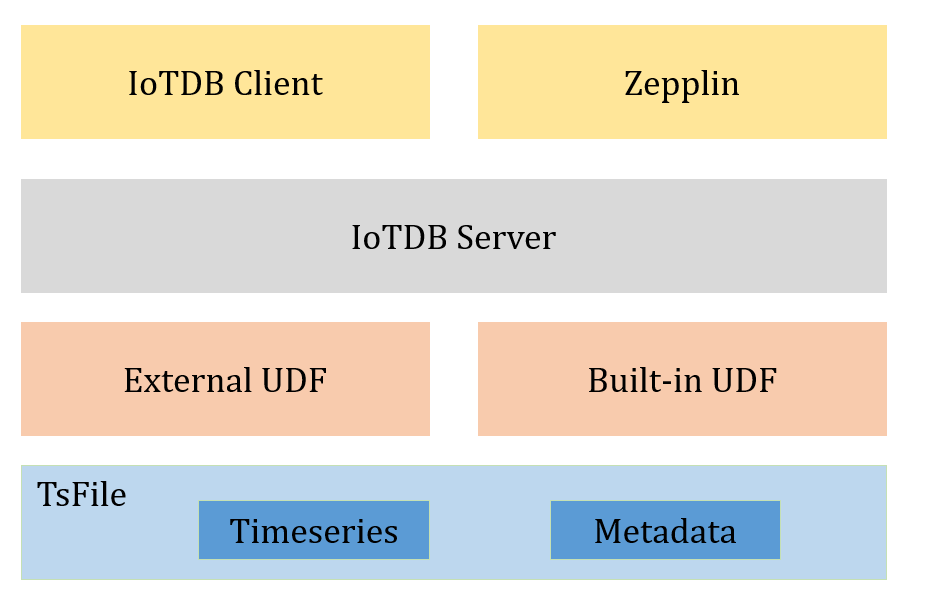
\includegraphics[width=0.66\linewidth]{udf-structure.PNG}
    \caption{基于IoTDB实现的对称子段判定和挖掘算法架构图}
    \label{fig:symmetry_structure}
\end{figure}

% IoTDB为用户提供了一套成熟的函数管理和执行框架,本文的算法实现即基于此框架。
Apache IoTDB为用户提供了一套成熟的函数管理和执行框架,
其底层存储方式也非常方便用户对查询计算功能进行扩展。
如图~\ref{fig:symmetry_structure}所示,IoTDB的数据存储
文件TsFile中不仅存储了时间序列,还存储了与计算查询相关的元数据信息。
根据算法流程对这些数据进行有选择地应用,即可实现原生UDF和
外部UDF两种不同的计算函数。最终这两类UDF都会整合到
IoTDB Server中为用户提供相关的数据分析功能,并将结果
由命令行客户端或Apache UI工具Zepplin进行展示。
根据对称子段判定和挖掘算法的计算方式和数据依赖,
本章对全局算法实现了只基于原始时序数据的外部UDF,
而对分段算法则实现了外部UDF和基于元数据的原生UDF两类函数,
尽可能满足不同场景用户的计算需求。


\section{对称子段判定算法实现}
IoTDB为用户提供了一个用于时间序列数据分析的自定义模板函数接口UDTF
(User Defined Timeseries Generating Function),
该模板支持多条时间序列和多个参数的输入,最终会输出一条时间序列数据
表示函数计算的结果。对于对称子段判定算法而言,根据
图~\ref{fig:global_algorithm_process}所示的计算流程,
只需要输入一条时间序列子段数据用于判定是否为对称子段,具体的
对称度和阈值都可以在函数处理中由算法计算。
在具体实现中,为方便用户使用,本算法提供了阈值(threshold)参数,
可以由领域专家自行指定对称度阈值,若不指定,则采用对称度阈值确定算法进行计算。
\begin{figure}
    \centering
    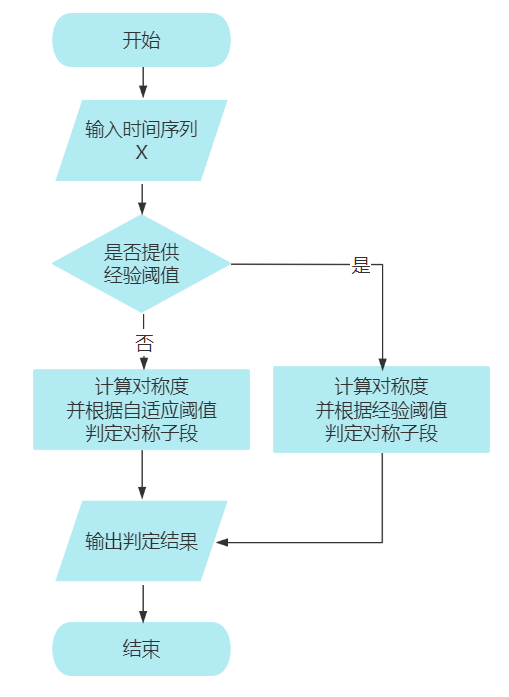
\includegraphics[width=0.55\linewidth]{global_symmetry_algorithm.PNG}
    \caption{基于IoTDB的对称子段判定算法流程图}
    \label{fig:global_algorithm_process}
\end{figure}

本算法用到了UDTF中定义的四个接口,具体实现方式如下所示:
\begin{itemize}
\item validate:验证算法的参数是否输入正确,threshold代表时间序列的
      对称度,一定是正数。如果不输入,则代表使用自定义的对称度阈值确定算法。
\item beforeStart:指定滑动窗口的数据访问策略并执行算法的初始化。由于
      对称子段判定算法是对子段整体计算对称性的,因此,设定子段的
      窗口大小为无穷大以将全部数据加载到算法中。
\item transform:执行全局算法以判定对称子段,具体步骤如下所示:
    \begin{enumerate}
        \item 对长度小于2的时间子段的对称度进行初始化计算。
        \item 按照长度由小到大的顺序推导并计算每一段时间子序列的对称度,并将结果
              保存在预定义的数据结构中。
        \item 根据时间序列子段的数据特征进行差分计算,得到单一对称度阈值。
        \item 由计算得到的对称度和对称度阈值判定输入时间序列子段是否属于对称子段。
    \end{enumerate}
\item terminate:将全局时间序列是否具有对称性的判定结果输出到collector中。
\end{itemize}

\section{对称子段挖掘算法实现}

对称子段挖掘算法的处理过程和对称子段判定算法有所不同,
挖掘算法是通过对时间序列进行分段从而分别挖掘对称子段的。
结合IoTDB将整条时间序列数据划分为不同的Chunk和Page进行存储,
并在计算时分段计算再合并结果的处理方式,分段算法和IoTDB的存储
计算框架高度契合。正因如此,分段算法既可以像对称子段判定算法一样
以外部UDF的方式完成计算,也可以利用每个Page的元数据加速计算。
对称子段挖掘算法的外部UDF实现方式非常简单,
直接利用算法~\ref{alg:symmetric_pattern}计算即可。
但分段算法的原生UDF实现方式却需要在计算时考虑元数据,
计算流程较为复杂。

\begin{figure}
    \centering
    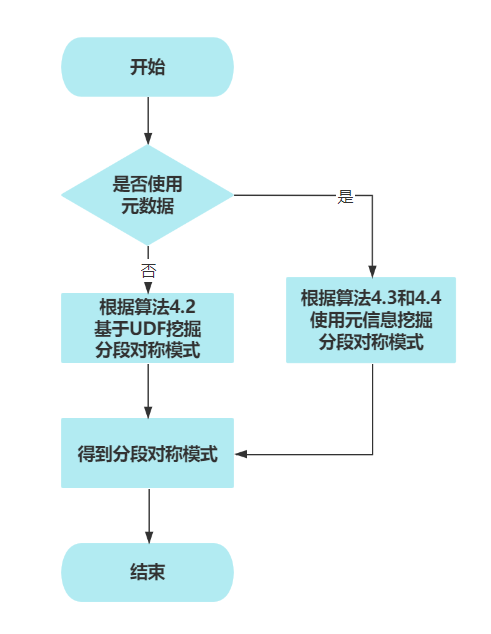
\includegraphics[width=0.55\linewidth]{iotdb_segement_symmetry.PNG}
    \caption{基于IoTDB的对称子段挖掘算法流程图}
    \label{fig:iotdb_segement}
  \end{figure}

图~\ref{fig:iotdb_segement}展示了基于IoTDB的对称子段
挖掘算法流程。算法在读入时间序列$X$和子序列长度约束$w$之后,
首先需要判断是否存在可以利用的元数据。
元数据的可用性必须满足三个条件,一是
在写入时已完成元数据计算并持久化到TsFile中,
二是写入时从系统配置中读取的子序列长度约束必须和输入的约束$w$
相同,三是查询的范围必须包含完整Page。
经过可用性检验,如果有对应的元数据,则直接合并元数据
就可以得到对称子段的数量。
反之,则还需要重新根据算法4.2加载原始时间序列并挖掘
对称子段。最终,算法输出对称子段挖掘得到的数量结果。

\section{算法查询展示}

在实现了对称子段判定和挖掘的算法逻辑之后,用户可以使用两种方式
执行算法并对结果进行查询。一种是利用IoTDB-Client命令行,
另一种是在Apache Zepplin上通过前端UI进行查询。
以对称子段判定算法为例,
在命令行上,用户登录客户端之后,直接输入调用UDF函数的SQL语句
进行查询,查询结果如图~\ref{fig:iotdb_client_symptn}所示。
直接使用Select语句就可以查询对称子段判定和挖掘结果。
使用IoTDB Client命令行进行查询的好处是查询便捷,
直接登录客户端即可查询,不需要重新部署其他工具。
但是,在命令行查询的结果只能通过表格的方式
进行展示,不方便直观的观察查询结果。仅通过在命令行中观察,
用户无法区分~\ref{fig:gsymptn_input}所示的查询数据是否
具有对称性,因而更无法对查询结果的正确性进行判断。
基于此,在IoTDB-Client上进行查询只适用于开发中的结果验证,
不适合商业化用户使用。因此,需要配置部署一个直观的前端查询方式。
\begin{figure}
    \centering
    \subcaptionbox{GunPointAgeSpan数据集\label{fig:gsymptn_input}}
    {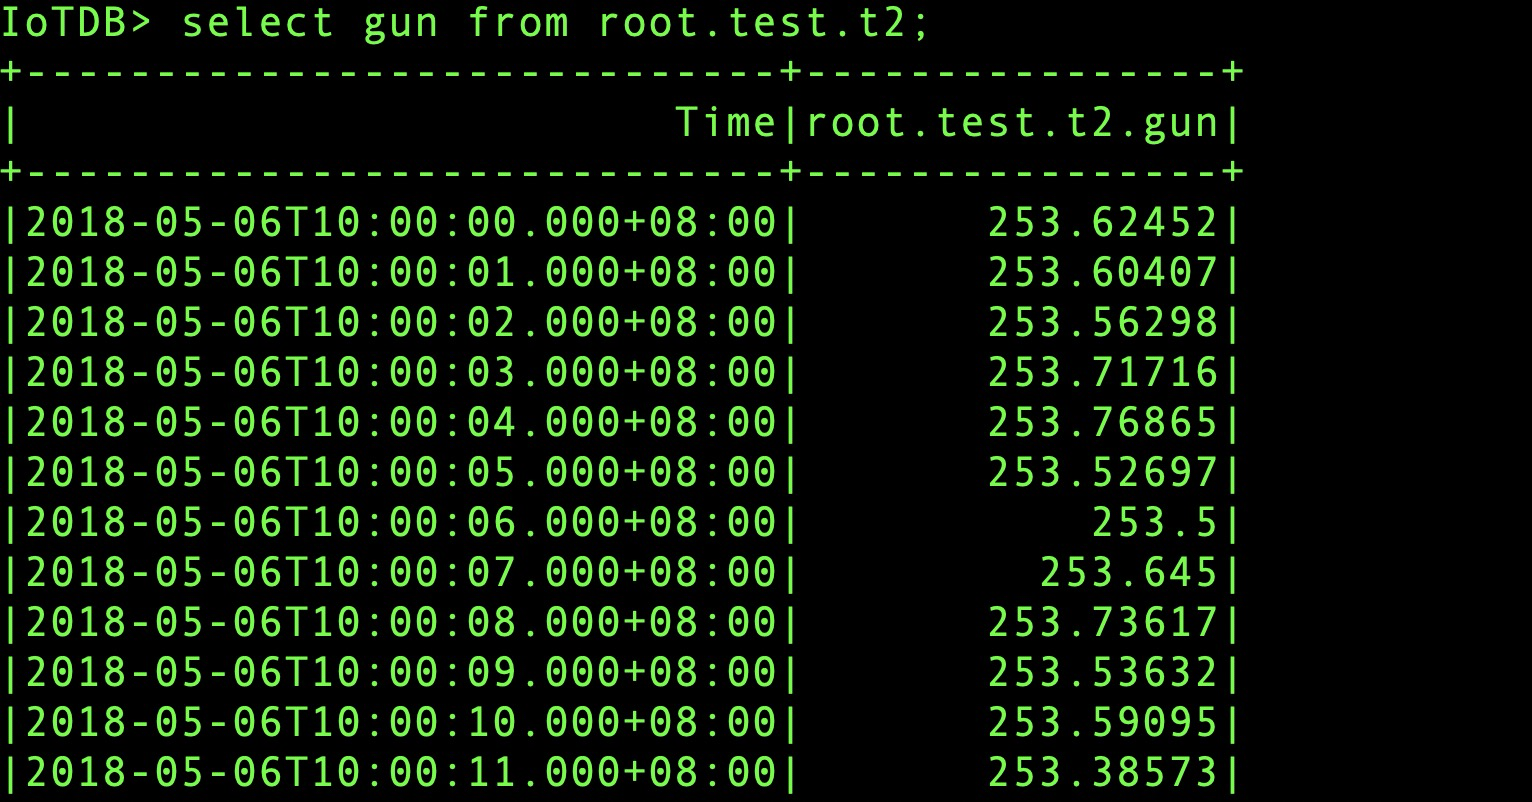
\includegraphics[width=0.76\linewidth]{gun_point_system.png}}
    \subcaptionbox{对称子段查询结果\label{fig:gsymptn_output}}
    {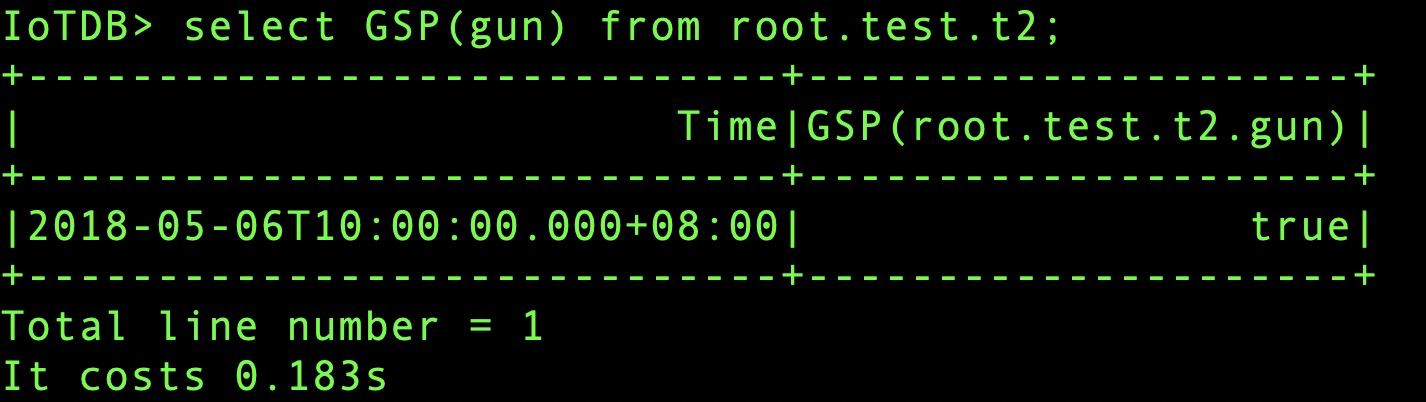
\includegraphics[width=0.76\linewidth]{gun_point_system_result.png}}
    \caption{在IoTDB-Client运行对称子段判定算法的结果查询展示}
    \label{fig:iotdb_client_symptn}
\end{figure}

Apache Zepplin是一个基于网页的交互式数据分析系统。
用户可以通过Zeppelin连接IoTDB数据源并使用SQL进行交互式查询操作。
图~\ref{fig:iotdb_zepplin_symptn}中展示了在Zepplin上进行
对称子段判定和挖掘结果计算并查询的方式,
图中上半部分是在运输车轨迹GPS经度
数据集随时间的变化情况。利用Zepplin自带的折线图
用户可以方便地观察出运输车轨迹数据集中的时间序列具有
16个对称子段。
图中下半部分是在运输车轨迹数据集上挖掘对称子段,
在Zepplin的输入框中直接输入Select语句
就可以像IoTDB-Client命令行一样执行查询,
发现算法的计算结果和真实结果一致。
\begin{figure}
    \centering
    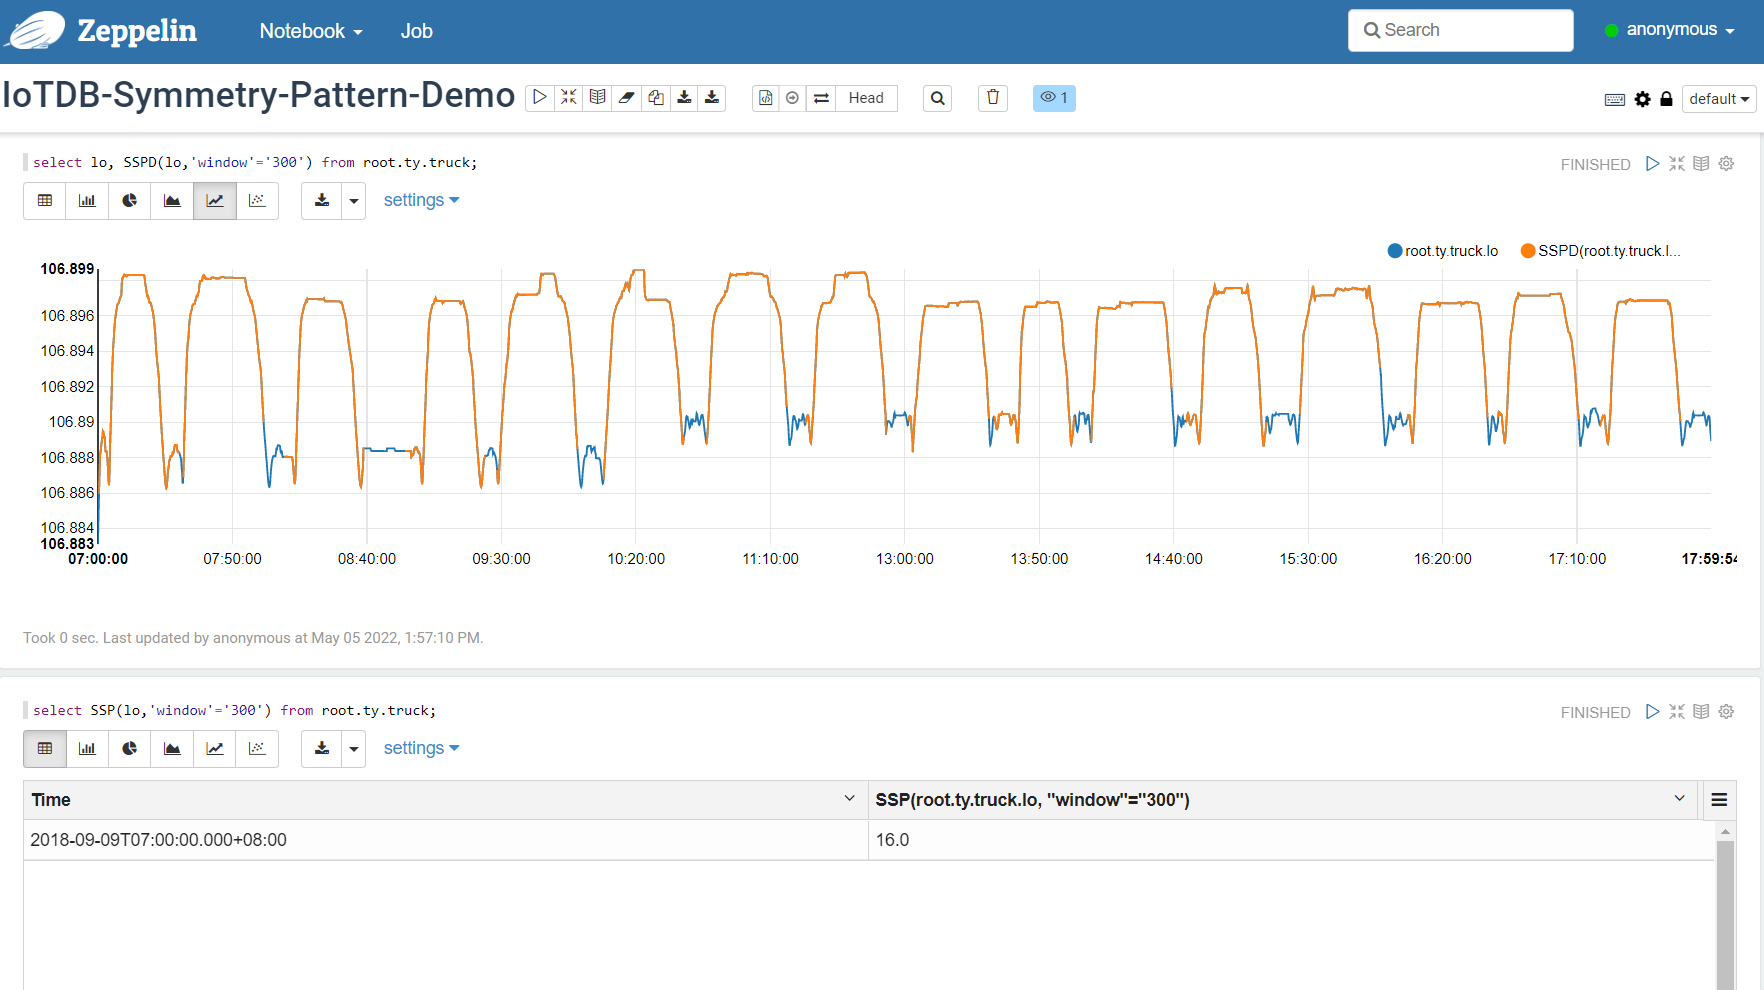
\includegraphics[width=0.85\linewidth]{zepplin_truck_data.PNG}
    \caption{在Apache zepplin运行对称子段挖掘算法的结果查询展示}
    \label{fig:iotdb_zepplin_symptn}
\end{figure}


\section{本章小结}
本章主要介绍了根据IoTDB提供的用户自定义函数模板接口,
对称子段判定和挖掘算法的实现方式,
并通过在IoTDB Server上进行部署,使用IoTDB Client和
Apache Zepplin两种方式进行函数调用计算和结果查询。
基于IoTDB实现这两种算法,弥补了IoTDB-Quality挖掘对称子段
的功能缺失,在帮助用户得到蕴含在时间序列中对称子段的同时,
便于发现违反规律的异常点并进行检测和修复。